
\chapter{Especificação}\label{chp:espec}
\section{Requisitos}\label{sec:req}

\subsection{Requisitos Funcionais}
- Enviar dados sobre a intensidade dos sinais de \textit{Wi-fi} ao servidor. \par
- Retornar a posição do usuário baseado nos dados enviados.\par
- Disponibilizar uma API para ser usada por outras aplicações.\par


\subsection{Requisitos Não-Funcionais}

- O sistema deve ser transparente ao usuário.\par


\section{Arquitetura e Fluxo de Dados}


O sistema possui a seguinte arquitetura, de acordo com o diagrama a seguir:


\begin{figure}[H]
	\centering
	\caption{Diagrama da Arquitetura do Sistema net.map}
  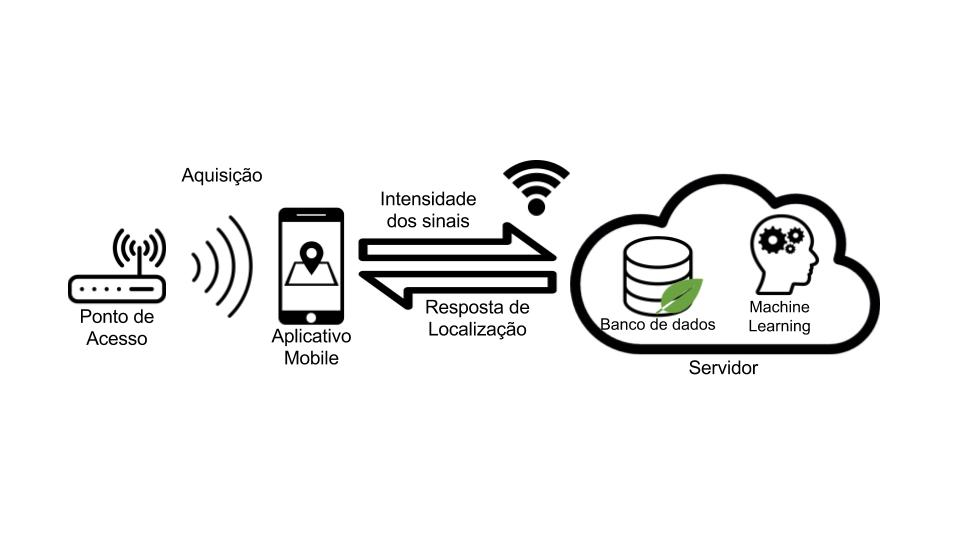
\includegraphics[width=0.9\textwidth]{Diagrama-arquitetura}
\label{fig:diagramaarq}

\end{figure}



\begin{figure}[H]
	\centering
	\caption{Fluxo de Dados do Sistema net.map}
  \includegraphics[width=0.9\textwidth]{diagramafluxodedados}
\label{fig:diagramafluxo}

\end{figure}


\section{Casos de Uso}

\subsection{Captura e Treinamento}

No primeiro caso de uso do sistema net.map, temos um usuário desejando mapear um ambiente. 


\subsection{Localização}